% Bachelor's thesis draft (Persian, XePersian). Compile with XeLaTeX from this folder:
%   xelatex main.tex   (twice, for the table of contents and references)
% Fonts: Estedad (fonts/, from github.com/aminabedi68/Estedad, SIL OFL).
% Numbers, tables and chart data come from scripts/make_reports.py (../tables, ../data).
\documentclass[12pt,a4paper,oneside]{report}
\usepackage[top=3cm,bottom=3cm,right=3cm,left=2.5cm]{geometry}
\usepackage{graphicx}
\usepackage{booktabs}
\usepackage{adjustbox}
\usepackage{caption}
\usepackage{pgfplots}
\pgfplotsset{compat=1.18, table/col sep=comma}
\usepackage[colorlinks=true,linkcolor=blue!50!black,citecolor=blue!50!black,urlcolor=blue!50!black]{hyperref}
\usepackage{xepersian}
\settextfont[Path=fonts/, BoldFont=Estedad-Bold.ttf]{Estedad-Regular.ttf}
\setdigitfont[Path=fonts/, BoldFont=Estedad-Bold.ttf]{Estedad-Regular.ttf}
\linespread{1.45}
\exhyphenpenalty=10000
\graphicspath{{../figures/}}
\captionsetup{font=small}
% Generated by scripts/make_reports.py: numbers quoted in the chapters.
\newcommand{\dataChips}{\LRE{112٬917}}
\newcommand{\dataScenes}{\LRE{422}}
\newcommand{\dataPasses}{\LRE{844}}
\newcommand{\dataTrainDark}{\LRE{1٬603}}
\newcommand{\testFOneCfar}{\LRE{0٫808}}
\newcommand{\testFOneRunOne}{\LRE{0٫763}}
\newcommand{\testFOneModel}{\LRE{0٫817}}
\newcommand{\testFOneNbCfar}{\LRE{0٫848}}
\newcommand{\testFOneNbModel}{\LRE{0٫854}}
\newcommand{\testDiff}{\LRE{+0٫009}}
\newcommand{\testDiffCi}{\LRE{+0٫002} تا \LRE{+0٫016}}
\newcommand{\testDiffNb}{\LRE{+0٫006}}
\newcommand{\testDiffNbCi}{\LRE{0٫000} تا \LRE{+0٫013}}
\newcommand{\darkRecallCfar}{\LRE{0٫77}}
\newcommand{\darkRecallRunOne}{\LRE{0٫50}}
\newcommand{\darkRecallModel}{\LRE{0٫81}}
\newcommand{\testRefs}{\LRE{3٬900}}
\newcommand{\testRefsDark}{\LRE{246}}
\newcommand{\genUaeTestStdModel}{\LRE{0٫817}}
\newcommand{\genUaeTestStdCfar}{\LRE{0٫808}}
\newcommand{\genUaeTestStdDiff}{\LRE{+0٫009}}
\newcommand{\genUaeTestStdCi}{\LRE{+0٫002} تا \LRE{+0٫016}}
\newcommand{\genUaeTestStdPrecision}{\LRE{0٫723}}
\newcommand{\genUaeTestStdRecall}{\LRE{0٫938}}
\newcommand{\genUaeTestFarModel}{\LRE{0٫817}}
\newcommand{\genUaeTestFarCfar}{\LRE{0٫812}}
\newcommand{\genUaeTestFarDiff}{\LRE{+0٫005}}
\newcommand{\genUaeTestFarCi}{\LRE{−0٫001} تا \LRE{+0٫013}}
\newcommand{\genUaeTestFarPrecision}{\LRE{0٫724}}
\newcommand{\genUaeTestFarRecall}{\LRE{0٫938}}
\newcommand{\genUaeEarlyStdModel}{\LRE{0٫827}}
\newcommand{\genUaeEarlyStdCfar}{\LRE{0٫833}}
\newcommand{\genUaeEarlyStdDiff}{\LRE{−0٫006}}
\newcommand{\genUaeEarlyStdCi}{\LRE{−0٫022} تا \LRE{+0٫008}}
\newcommand{\genUaeEarlyStdPrecision}{\LRE{0٫739}}
\newcommand{\genUaeEarlyStdRecall}{\LRE{0٫938}}
\newcommand{\genUaeEarlyFarModel}{\LRE{0٫827}}
\newcommand{\genUaeEarlyFarCfar}{\LRE{0٫835}}
\newcommand{\genUaeEarlyFarDiff}{\LRE{−0٫008}}
\newcommand{\genUaeEarlyFarCi}{\LRE{−0٫023} تا \LRE{+0٫006}}
\newcommand{\genUaeEarlyFarPrecision}{\LRE{0٫739}}
\newcommand{\genUaeEarlyFarRecall}{\LRE{0٫938}}
\newcommand{\genUaeNewStdModel}{\LRE{0٫721}}
\newcommand{\genUaeNewStdCfar}{\LRE{0٫718}}
\newcommand{\genUaeNewStdDiff}{\LRE{+0٫003}}
\newcommand{\genUaeNewStdCi}{\LRE{−0٫006} تا \LRE{+0٫014}}
\newcommand{\genUaeNewStdPrecision}{\LRE{0٫591}}
\newcommand{\genUaeNewStdRecall}{\LRE{0٫924}}
\newcommand{\genUaeNewFarModel}{\LRE{0٫721}}
\newcommand{\genUaeNewFarCfar}{\LRE{0٫722}}
\newcommand{\genUaeNewFarDiff}{\LRE{0٫000}}
\newcommand{\genUaeNewFarCi}{\LRE{−0٫009} تا \LRE{+0٫011}}
\newcommand{\genUaeNewFarPrecision}{\LRE{0٫591}}
\newcommand{\genUaeNewFarRecall}{\LRE{0٫924}}
\newcommand{\genIranTestStdModel}{\LRE{0٫781}}
\newcommand{\genIranTestStdCfar}{\LRE{0٫674}}
\newcommand{\genIranTestStdDiff}{\LRE{+0٫108}}
\newcommand{\genIranTestStdCi}{\LRE{+0٫085} تا \LRE{+0٫137}}
\newcommand{\genIranTestStdPrecision}{\LRE{0٫673}}
\newcommand{\genIranTestStdRecall}{\LRE{0٫932}}
\newcommand{\genIranTestFarModel}{\LRE{0٫795}}
\newcommand{\genIranTestFarCfar}{\LRE{0٫780}}
\newcommand{\genIranTestFarDiff}{\LRE{+0٫015}}
\newcommand{\genIranTestFarCi}{\LRE{+0٫002} تا \LRE{+0٫030}}
\newcommand{\genIranTestFarPrecision}{\LRE{0٫693}}
\newcommand{\genIranTestFarRecall}{\LRE{0٫931}}
\newcommand{\genIranNewStdModel}{\LRE{0٫644}}
\newcommand{\genIranNewStdCfar}{\LRE{0٫491}}
\newcommand{\genIranNewStdDiff}{\LRE{+0٫152}}
\newcommand{\genIranNewStdCi}{\LRE{+0٫113} تا \LRE{+0٫207}}
\newcommand{\genIranNewStdPrecision}{\LRE{0٫499}}
\newcommand{\genIranNewStdRecall}{\LRE{0٫905}}
\newcommand{\genIranNewFarModel}{\LRE{0٫652}}
\newcommand{\genIranNewFarCfar}{\LRE{0٫631}}
\newcommand{\genIranNewFarDiff}{\LRE{+0٫022}}
\newcommand{\genIranNewFarCi}{\LRE{+0٫004} تا \LRE{+0٫047}}
\newcommand{\genIranNewFarPrecision}{\LRE{0٫509}}
\newcommand{\genIranNewFarRecall}{\LRE{0٫909}}
\newcommand{\darkVal}{\LRE{4٫0}٪}
\newcommand{\darkUaeTest}{\LRE{4٫0}٪}
\newcommand{\darkUaeEarly}{\LRE{27٫8}٪}
\newcommand{\darkUaeNew}{\LRE{7٫9}٪}
\newcommand{\persistPrecisionBefore}{\LRE{0٫509}}
\newcommand{\persistPrecisionAfter}{\LRE{0٫523}}
\newcommand{\testModelSeconds}{\LRE{14٫4}}
\newcommand{\benchSeconds}{\LRE{8٫4}}
\newcommand{\benchMemory}{\LRE{209}}
\newcommand{\benchWindow}{\LRE{2٬000}}


\begin{document}

\begin{titlepage}
\centering
\vspace*{2cm}
{\large [نام دانشگاه]\par}
{\large [دانشکده و گروه]\par}
\vspace{1.5cm}
{\large پایان‌نامه کارشناسی\par}
\vspace{1.5cm}
{\LARGE\bfseries آشکارسازی شناورها در تصاویر راداری \lr{Sentinel-1} در خلیج فارس با یادگیری عمیق و یافتن شناورهای تاریک\par}
\vspace{2cm}
{\large نگارنده: [نام دانشجو]\par}
\vspace{0.5cm}
{\large استاد راهنما: [نام استاد راهنما]\par}
\vfill
{\large [ماه و سال]\par}
\end{titlepage}

\pagenumbering{alph}
\chapter*{چکیده}
خلیج فارس و تنگه هرمز از پرترددترین آبراه‌های جهان‌اند، اما سامانه شناسایی خودکار
(\lr{AIS})، که شناورها موقعیت خود را با آن اعلام می‌کنند، خوداظهاری است: می‌توان آن را
خاموش یا جعل کرد. تصاویر رادار روزنه مصنوعی (\lr{SAR}) ماهواره \lr{Sentinel-1} شناور را
بی‌توجه به \lr{AIS}، ابر و شب می‌بینند. در این پژوهش یک آشکارساز نقطه‌ای یادگیری عمیق
(رمزگذار \lr{EfficientNet-B0} و رمزگشای \lr{U-Net}) بدون برچسب‌گذاری دستی و با برچسب‌هایی
که از آشکارسازی‌های راداری \lr{Global Fishing Watch} (\lr{GFW}) ساخته شد آموزش دید و روی
پردازنده یک رایانه همراه اجرا شد. نخستین مدل شناورهای بدون \lr{AIS} را کمتر از روش کلاسیک
\lr{CFAR} می‌یافت (بازیابی \darkRecallRunOne{} در برابر \darkRecallCfar)، زیرا برچسب‌ها تنها
از شناورهای دارای \lr{AIS} آمده بود؛ افزودن آشکارسازی‌های بدون \lr{AIS} به نمونه‌های مثبت
این سوگیری را برطرف کرد (\darkRecallModel). روی ۹۲ گذر آزمون نگه‌داشته، \lr{F1} مدل نهایی
در برابر \lr{GFW} برابر \testFOneModel{} و \lr{CFAR} برابر \testFOneCfar{} بود (تفاضل
\testDiff، بازه ۹۵٪: \testDiffCi). مدل بدون بازتنظیم به ماهواره‌های تازه \lr{Sentinel-1C/1D}
و به ساحل ایران تعمیم یافت. با تلفیق آشکارسازی‌ها با حضور ساعتی \lr{AIS}، نامزدهای شناور
تاریک همراه شواهدشان مشخص شد و همه در یک کنسول وب فارسی، هر کدام با تصویر راداری‌اش،
نمایش داده می‌شود.

\noindent\textbf{واژگان کلیدی:} رادار روزنه مصنوعی، \lr{Sentinel-1}، یادگیری عمیق،
آشکارسازی شناور، شناور تاریک، \lr{AIS}، خلیج فارس.

\tableofcontents
\listoftables
\listoffigures
\cleardoublepage
\pagenumbering{arabic}

\chapter{مقدمه}
\label{ch:intro}

\section{بیان مسئله}
خلیج فارس، تنگه هرمز و دریای عمان گذرگاه بخش بزرگی از نفت و کالای دریایی جهان‌اند. برای
پایش این آبراه‌ها، داده اصلی امروز سامانه شناسایی خودکار (\lr{AIS}) است: هر شناورِ مشمول
مقررات، شناسه، موقعیت، سرعت و جهت خود را به‌طور منظم پخش می‌کند و گیرنده‌های ساحلی و
ماهواره‌ای این پیام‌ها را جمع می‌کنند. اما \lr{AIS} خوداظهاری است: شناور می‌تواند فرستنده را
خاموش کند، موقعیت ساختگی بفرستد یا در منطقه‌ای باشد که اخلال در ناوبری ماهواره‌ای
(\lr{GNSS}) موقعیتش را جابه‌جا می‌کند. شناوری که در دریا هست ولی در \lr{AIS} دیده نمی‌شود را
«شناور تاریک» می‌نامند.

تصاویر رادار روزنه مصنوعی (\lr{SAR}) راه مستقلی برای دیدن شناورهاست. رادار خود انرژی
می‌فرستد و بازتاب آن را می‌گیرد، پس در شب و از پشت ابر هم تصویر می‌گیرد، و بدنه فولادی
شناور در آن به‌صورت نقطه‌ای روشن روی دریای تیره دیده می‌شود، چه شناور \lr{AIS} داشته باشد چه
نه. ماهواره‌های \lr{Sentinel-1} برنامه کوپرنیک اروپا این تصاویر را به‌رایگان و با تفکیک حدود
۱۰ متر در دسترس می‌گذارند. پرسش این پژوهش این است که یک مدل یادگیری عمیق تا چه اندازه
می‌تواند شناورها را در این تصاویر بیابد، چگونه می‌توان آن را بدون برچسب‌گذاری دستی آموزش
داد، دقتش را در برابر مرجعی مستقل سنجید، و از کنار هم گذاشتن آشکارسازی‌های راداری با
\lr{AIS} نامزدهای شناور تاریک را با شواهدشان یافت.

\section{هدف‌ها}
\begin{enumerate}
\item آموزش یک آشکارساز یادگیری عمیق برای یافتن شناور در تصاویر \lr{Sentinel-1} بدون
برچسب‌گذاری دستی، که روی پردازنده یک رایانه همراه اجرا شود.
\item سنجش آن در برابر مرجعی مستقل، یعنی آشکارسازی‌های راداری منتشرشده
\lr{Global Fishing Watch} (\lr{GFW})، و مقایسه با روش کلاسیک \lr{CFAR} روی گذرهایی که در
آموزش و انتخاب مدل به کار نرفته‌اند.
\item آزمودن تعمیم مدل به زمانی دیگر، به ماهواره‌های تازه \lr{Sentinel-1C/1D} و به منطقه‌ای
دیگر (ساحل ایران).
\item یافتن نامزدهای شناور تاریک با تلفیق آشکارسازی‌ها با حضور ساعتی \lr{AIS} و ثبت شواهد
هر نامزد.
\item ساخت یک کنسول وب که هر آشکارسازی را همراه تصویر راداری‌اش و با بیان صادقانه سن داده و
دقت سنجیده‌شده نشان دهد.
\end{enumerate}

\section{دستاوردها}
\begin{itemize}
\item \textbf{برچسب‌گذاری خودکار:} برچسب‌های آموزشی از تطبیق آشکارسازی‌های \lr{CFAR} با
خانه‌های آشکارسازی \lr{GFW} ساخته شد (\dataChips{} برش تصویری از \dataScenes{} تصویر).
\item \textbf{سوگیری برچسب و رفع آن:} مدل نخست، که فقط شناورهای دارای \lr{AIS} را مثبت
می‌دید، شناورهای بدون \lr{AIS} را کمتر از \lr{CFAR} می‌یافت (بازیابی \darkRecallRunOne{} در
برابر \darkRecallCfar). افزودن \dataTrainDark{} آشکارسازی بدون \lr{AIS} به نمونه‌های مثبت
بازیابی را به \darkRecallModel{} رساند.
\item \textbf{سنجش نگه‌داشته:} روی ۹۲ گذر آزمون، \lr{F1} مدل نهایی \testFOneModel{} و
\lr{CFAR} \testFOneCfar{} بود؛ پیکربندی مدل فقط روی گذرهای اعتبارسنجی برگزیده شد.
\item \textbf{تعمیم:} مدل بدون بازتنظیم روی \lr{Sentinel-1C/1D} و ساحل ایران کار کرد؛ برتری
ظاهری بزرگ آن بر \lr{CFAR} نزدیک ساحل به نوار یک‌کیلومتری‌ای برمی‌گردد که \lr{GFW} در آن
گزارشی ندارد، و دورتر از ساحل برتری کوچک اما معنادار می‌ماند.
\item \textbf{شناورهای تاریک:} تلفیق خانه-ساعت با حضور \lr{AIS} نرخ نامزد تاریک را در دوره‌ها و
منطقه‌های گوناگون با روشی یکسان می‌سنجد و هر نامزد را با شواهدش ثبت می‌کند.
\item \textbf{سامانه:} زنجیره‌ای از خواندن تصویر تا کنسول وب فارسی و راست‌به‌چپ، که هر
آشکارسازی را با تصویر راداری‌اش نشان می‌دهد.
\end{itemize}

\section{ساختار گزارش}
فصل~\ref{ch:background} مبانی رادار، \lr{AIS} و پیشینه آشکارسازی شناور را مرور می‌کند.
فصل~\ref{ch:method} داده‌ها، برچسب‌گذاری خودکار، مدل، روش سنجش و تلفیق با \lr{AIS} را شرح
می‌دهد. فصل~\ref{ch:results} نتایج را می‌آورد و فصل~\ref{ch:conclusion} به بحث، محدودیت‌ها و
کارهای آینده می‌پردازد.

\chapter{مبانی و پیشینه}
\label{ch:background}

\section{رادار روزنه مصنوعی و \lr{Sentinel-1}}
رادار روزنه مصنوعی (\lr{SAR}) پالس‌های ریزموج به سطح زمین می‌فرستد و بازتاب آن‌ها را ثبت
می‌کند؛ با پردازش سیگنال در طول مسیر ماهواره، تفکیکی به دست می‌آید که با آنتنی واقعی
ناممکن بود. سطح آرام دریا بیشتر انرژی را دور از ماهواره بازمی‌تاباند و تیره دیده می‌شود، اما
بدنه و سازه فولادی شناور مانند بازتابنده‌ای گوشه‌ای عمل می‌کند و نقطه‌ای روشن پدید می‌آورد.

مأموریت \lr{Sentinel-1} \cite{torres2012} تصاویر باند \lr{C} را در حالت پهنای گسترده
(\lr{IW}) با نوار حدود ۲۵۰ کیلومتر برمی‌دارد. در این پژوهش محصول \lr{GRD} با پیکسل ۱۰ متر و
دو قطبش \lr{VV} و \lr{VH} به کار رفت؛ شناور در قطبش متقاطع \lr{VH} معمولاً تضاد بیشتری با دریا
دارد. تصاویر از زیرساخت \lr{Copernicus Data Space Ecosystem} \cite{cdse} و به قالب
\lr{Cloud-Optimized GeoTIFF} خوانده شد، که خواندن تنها پنجره مورد نیاز را بدون بارگیری کل
تصویر ممکن می‌کند. در دوره این پژوهش ماهواره‌های \lr{Sentinel-1C} و \lr{Sentinel-1D} جای
\lr{Sentinel-1A} را گرفتند؛ ازاین‌رو تعمیم مدل به این ماهواره‌ها جداگانه سنجیده شد.

\section{سامانه شناسایی خودکار و \lr{Global Fishing Watch}}
\lr{AIS} برای ایمنی ناوبری طراحی شد و شناور شناسه (\lr{MMSI})، موقعیت، سرعت و جهتش را
پخش می‌کند. پوشش، صداقت و پیوستگی آن تضمین‌شده نیست: فرستنده ممکن است خاموش شود و
موقعیت‌ها ممکن است جعل یا با اخلال \lr{GNSS} جابه‌جا شوند. \lr{Global Fishing Watch} داده‌های
\lr{AIS} را در مقیاس جهانی پردازش می‌کند \cite{kroodsma2018} و آشکارسازی‌های شناور در تصاویر
\lr{Sentinel-1} را با \lr{AIS} تطبیق می‌دهد \cite{paolo2024}. این پژوهش از دو داده عمومی آن
استفاده کرد \cite{gfwapi}: آشکارسازی‌های راداری (با و بدون تطبیق \lr{AIS}) در خانه‌های
\LRE{0٫01} درجه‌ای (حدود ۱ کیلومتر) و ساعتی، و حضور ساعتی شناورهای \lr{AIS} در همان خانه‌ها.
\lr{GFW} سازه‌های ثابت را جدا می‌کند و در نوار نزدیک ساحل آشکارسازی گزارش نمی‌کند؛ این دو
نکته در فصل نتایج اهمیت می‌یابند.

\section{آشکارسازی کلاسیک: \lr{CFAR}}
روش کلاسیک آشکارسازی شناور در \lr{SAR}، آشکارساز با نرخ هشدار نادرست ثابت (\lr{CFAR}) است
\cite{crisp2004}. برای هر پیکسل، میانگین بازتاب دریا در حلقه‌ای از پیکسل‌های آموزشی پیرامون آن
برآورد می‌شود (با نواری محافظ تا انرژی خود هدف برآورد را آلوده نکند) و پیکسلی که از مضربی از
این میانگین روشن‌تر باشد آشکار شمرده می‌شود. مضرب از آماره دریا و نرخ هشدار نادرست
دلخواه به دست می‌آید. \lr{CFAR} به داده آموزشی نیاز ندارد و پارامترهایش تفسیرپذیرند، پس
خط مبنای مناسبی است؛ اما بازتاب سازه‌ها، ساحل و نوارهای اثر رادار را نیز آشکار می‌کند و
شناورهای بزرگ را گاه به چند تکه می‌شکند.

\section{یادگیری عمیق برای آشکارسازی شناور}
مسابقه \lr{xView3} \cite{paolo2022} داده‌ای بزرگ از تصاویر \lr{Sentinel-1} با برچسب شناور و
وضعیت \lr{AIS} فراهم کرد. راه‌حل برنده \cite{xview3first} شناور را به‌جای جعبه مرزی، به‌صورت
نقطه آشکار می‌کرد: شبکه‌ای با رمزگذار از پیش آموزش‌دیده و رمزگشای \lr{U-Net}
\cite{ronneberger2015} برای هر پیکسل خروجی، احتمال مرکز شناور و جابه‌جایی زیرپیکسلی آن را
پیش‌بینی می‌کند، به روش «اشیا به‌مثابه نقطه» \cite{zhou2019}. این رویکرد برای اهدافی که در
تصویر تنها چند پیکسل‌اند مناسب‌تر از آشکارسازهای جعبه‌ای است. رمزگذار این پژوهش
\lr{EfficientNet-B0} \cite{tan2019} است و تابع زیان نقشه مرکز، زیان کانونی کاهش‌یافته
\cite{lin2017,zhou2019}.

\section{شناورهای تاریک و تلفیق داده‌ها}
یافتن شناور تاریک یعنی پیدا کردن آشکارسازی راداری‌ای که هیچ شناور \lr{AIS} در آن زمان و
مکان آن را توضیح ندهد. دشواری در جزئیات است: زمان گذر ماهواره و پیام‌های \lr{AIS} یکی نیست،
موقعیت‌ها خطا دارند، شناور میان پیام‌ها جابه‌جا می‌شود و چند شناور ممکن است به یک
آشکارسازی نزدیک باشند. این پژوهش تطبیق را به‌صورت تخصیص یک‌به‌یک
\cite{kuhn1955} میان آشکارسازی‌ها و «دروازه‌های» زمانی-مکانی شناورهای \lr{AIS} انجام داد
(بخش~\ref{sec:fusion}).

\chapter{داده‌ها و روش}
\label{ch:method}

\section{منطقه مطالعه}
پنج «محدوده مطالعاتی» در سوی امارات و تنگه هرمز انتخاب شد: فجیره، خورفکان، شارجه/دبی و
راس‌الخیمه (هر کدام مربعی ۲۰ کیلومتری) و آبراه هرمز (۴۰ کیلومتری). همه داده‌های آموزش،
اعتبارسنجی و آزمون از همین پنج محدوده آمد. برای سنجش تعمیم به منطقه‌ای تازه، هفت محدوده
۲۰ کیلومتری در ساحل ایران نیز تعریف شد: بندرعباس، لارک/هرمز، کیش، عسلویه، بوشهر، خارک و
جاسک (شکل~\ref{fig:map}). مدل هرگز روی داده این هفت محدوده آموزش ندید و پیکربندی‌اش بر پایه
آن‌ها انتخاب نشد.

\begin{figure}[htbp]
\centering
\begin{tikzpicture}
\begin{axis}[
  width=0.95\textwidth, height=0.85\textwidth,
  xmin=47.5, xmax=60, ymin=23, ymax=30.6,
  unit vector ratio=0.895 1,
  unbounded coords=jump,
  axis background/.style={fill=blue!4},
  xlabel={\rl{طول جغرافیایی (درجه شرقی)}},
  ylabel={\rl{عرض جغرافیایی (درجه شمالی)}},
  tick label style={font=\footnotesize},
]
\addplot[gray!60!black, thin] table[x=lon, y=lat, col sep=comma] {../data/coast.csv};
\addplot[red!80!black, thick] table[x=lon, y=lat, col sep=comma] {../data/boxes.csv};
\node[font=\small, gray!40!black] at (axis cs:51.6,26.9) {\rl{خلیج فارس}};
\node[font=\small, gray!40!black] at (axis cs:58.6,24.3) {\rl{دریای عمان}};
\node[font=\scriptsize] at (axis cs:56.25,27.45) {\rl{بندرعباس}};
\node[font=\scriptsize] at (axis cs:50.3,29.65) {\rl{خارک}};
\node[font=\scriptsize] at (axis cs:53.98,26.15) {\rl{کیش}};
\node[font=\scriptsize] at (axis cs:57.8,25.2) {\rl{جاسک}};
\node[font=\scriptsize] at (axis cs:56.9,24.95) {\rl{فجیره}};
\node[font=\scriptsize] at (axis cs:55.3,25.05) {\rl{دبی}};
\end{axis}
\end{tikzpicture}
\caption[منطقه مطالعه]{منطقه مطالعه: پنج محدوده مطالعاتی امارات و تنگه هرمز (داده‌های آموزش و آزمون) و
هفت محدوده ساحل ایران (منطقه نگه‌داشته برای سنجش تعمیم). خط ساحل از \lr{OpenStreetMap}.}
\label{fig:map}
\end{figure}

\section{داده‌ها}
\begin{itemize}
\item \textbf{تصاویر راداری:} محصولات \lr{IW GRDH} ماهواره‌های \lr{Sentinel-1A}
(سال‌های ۲۰۲۴ و ۲۰۲۵ و نیمه نخست ۲۰۲۶) و \lr{Sentinel-1C/1D} (سپتامبر ۲۰۲۶) از \lr{CDSE}
\cite{cdse}؛ از هر تصویر تنها پنجره پیرامون محدوده خوانده شد.
\item \textbf{آشکارسازی‌های راداری و حضور \lr{AIS}:} از \lr{API} عمومی \lr{GFW} \cite{gfwapi}، در
خانه‌های \LRE{0٫01} درجه‌ای و ساعتی.
\item \textbf{خشکی:} چندضلعی‌های خشکی \lr{OpenStreetMap} \cite{osm}، با نوار حائل ۱۵۰ متری در دریا.
\item \textbf{سکوهای دریایی:} مجموعه \lr{Offshore Platform Dataset} \cite{spanier2026}، با طول عمر
هر سکو، تا سکوهای موجود در تاریخ هر تصویر پوشانده شوند.
\end{itemize}

\section{برچسب‌گذاری خودکار}
\label{sec:labels}
برچسب‌گذاری دستی هزاران شناور ممکن نبود؛ برچسب‌ها از کنار هم گذاشتن آشکارسازی‌های
\lr{CFAR} ما با آشکارسازی‌های \lr{GFW} در همان تصویر ساخته شد. چون \lr{GFW} داده را به‌صورت
شمارش در خانه‌های حدوداً یک‌کیلومتری منتشر می‌کند، آشکارسازی ما تنها وقتی برچسب گرفت که
خانه‌اش بی‌ابهام بود: دقیقاً یک شناور تطبیق‌یافته با \lr{AIS}، هیچ آشکارسازی بدون \lr{AIS}
و هیچ آشکارسازی دیگری از ما. آشکارسازی‌های نزدیک لبه خانه، اگر خانه همسایه چیزی داشت،
مبهم شمرده شدند. از هر آشکارسازی برشی ۱۲۸ پیکسلی (دو قطبش) ساخته شد. افزون بر مثبت‌ها،
برش‌های منفی از دریای خالی و برش‌هایی با ناحیه «نادیده» (اجسامی که برچسب مطمئن نداشتند)
ساخته شد؛ آشکارسازی بی‌برچسب هرگز منفی شمرده نشد. تقسیم آموزش، اعتبارسنجی و آزمون بر پایه
تصویر انجام شد، نه تصادفی، تا برش‌های مجاورِ یک تصویر میان بخش‌ها نشت نکنند
(جدول~\ref{tab:data}).

\begin{table}[htbp]
\centering
\small
\begin{adjustbox}{max width=\textwidth}
\begin{tabular}{lcccccc}
\toprule
بخش & تصویر & گذر-محدوده & مثبت با \lr{AIS} & مثبت بدون \lr{AIS} & منفی & نادیده \\
\midrule
آموزش & \LRE{329} & \LRE{649} & \LRE{17٬701} & \LRE{1٬603} & \LRE{53٬465} & \LRE{14٬293} \\
اعتبارسنجی & \LRE{51} & \LRE{103} & \LRE{2٬893} & \LRE{224} & \LRE{8٬302} & \LRE{2٬200} \\
آزمون & \LRE{42} & \LRE{92} & \LRE{2٬679} & \LRE{144} & \LRE{7٬307} & \LRE{2٬106} \\
\bottomrule
\end{tabular}
\end{adjustbox}
\caption[داده‌های آموزش، اعتبارسنجی و آزمون]{داده‌های آموزش، اعتبارسنجی و آزمون در پنج محدوده مطالعاتی (\lr{Sentinel-1A}، ۲۰۲۴ تا ۲۰۲۵). تقسیم بر پایه تصویر است، نه تصادفی. «مثبت بدون \lr{AIS}» آشکارسازی‌های \lr{GFW} بدون تطبیق \lr{AIS} است که در مدل نهایی مثبت گرفته شد.}
\label{tab:data}
\end{table}


\section{مدل}
مدل یک آشکارساز نقطه‌ای چگال است: رمزگذار \lr{EfficientNet-B0} \cite{tan2019} با وزن‌های
از پیش آموزش‌دیده \lr{ImageNet}، رمزگشای \lr{U-Net} \cite{ronneberger2015} و خروجی با گام ۲
(نیمی از تفکیک ورودی). دو سر خروجی دارد: نقشه احتمال مرکز شناور و جابه‌جایی زیرپیکسلی مرکز.
نقشه مرکز با زیان کانونی کاهش‌یافته \cite{lin2017,zhou2019} و جابه‌جایی با زیان \lr{L1} روی
پیکسل‌های مرکز آموزش دید؛ ناحیه‌های «نادیده» در زیان وزن صفر داشتند. سرهای طول، پهنا،
جهت و رده که در طرح اولیه بودند کنار گذاشته شدند، چون برچسب قابل‌اعتمادی برایشان نبود.

آموزش در \lr{Kaggle} روی یک \lr{GPU} مدل \lr{Tesla T4} انجام شد: ۱۵ دوره، هر دوره
\LRE{40٬000} نمونه وزن‌دار، دسته ۶۴ و نرخ یادگیری یک‌چرخه‌ای با بیشینه \LRE{0٫001}.
مدل نخست (\lr{run 1}) آشکارسازی‌های بدون \lr{AIS} را نادیده می‌گرفت. مدل نهایی
(\lr{run 2}) سه تفاوت داشت: آشکارسازی‌های بدون \lr{AIS} \lr{GFW} مثبت شمرده شدند، برش‌های
تصادفی ۹۶ پیکسلی از برش‌های ۱۲۸ پیکسلی به کار رفت تا شناور همیشه در مرکز نباشد، و وزن‌های
همه دوره‌ها نگه داشته شد. مدل به \lr{ONNX} با دقت \lr{fp32} صادر شد؛ کوانتش \lr{INT8}
خروجی‌ها را خراب می‌کرد و کنار گذاشته شد.

\section{استنتاج و انتخاب پیکربندی}
پنجره محدوده به کاشی‌های ۲۵۶ پیکسلی با هم‌پوشانی ۶۴ پیکسل تقسیم می‌شود، نقشه‌ها به هم
دوخته می‌شوند و بیشینه‌های محلی بالاتر از آستانه ۰٫۶۰ آشکارسازی‌اند. دوره آموزش، اندازه
کاشی و آستانه تنها روی ۲۵ گذر اعتبارسنجی و در برابر \lr{GFW} برگزیده شد
(جدول~\ref{tab:validation} در فصل نتایج)، با قاعده‌ای که پیش از دیدن هر عدد آزمون توافق شد:
بیشینه میانگین \lr{F1} دو قاعده تطبیق.

\section{روش سنجش}
\label{sec:evaluation}
برچسب‌های آموزشی خود از \lr{CFAR} آمده‌اند، پس \lr{CFAR} را نمی‌توان در برابر آن‌ها منصفانه
سنجید. مرجع مستقل، همه آشکارسازی‌های راداری \lr{GFW} (با و بدون \lr{AIS}) در محدوده و در ساعت
گذر است. چون \lr{GFW} شمارش هر خانه \LRE{0٫01} درجه‌ای را منتشر می‌کند، آشکارسازی‌ها در سطح
خانه تطبیق می‌یابند: آشکارسازی ما درست است اگر خانه‌اش هنوز آشکارسازی تطبیق‌نیافته‌ای از
\lr{GFW} داشته باشد («همان خانه»)؛ قاعده آسان‌گیرتر، خانه‌های همسایه را نیز می‌پذیرد. دقت،
بازیابی و \lr{F1} از این شمارش‌ها، و بازیابی جداگانه روی آشکارسازی‌های با و بدون \lr{AIS}
محاسبه می‌شود. همه آشکارسازها روی یک پنجره و با یک نقاب خشکی و سکو اجرا می‌شوند. تفاضل
مدل و \lr{CFAR} با بوت‌استرپ جفتی روی گذرها \cite{efron1993} و بازه ۹۵٪ گزارش می‌شود.

دو لایه افزوده، پیش از دیدن نتایج ساحل ایران تعریف شد: امتیازدهی تنها روی خانه‌هایی که مرکزشان
دست‌کم ۱ کیلومتر از خشکی فاصله دارد، زیرا \lr{GFW} در این نوار آشکارسازی گزارش نمی‌کند؛ و
زیرمجموعه گذرهایی که هیچ قابِ گذرشان در آموزش یا اعتبارسنجی نبوده است. \lr{GFW} حقیقت
زمینی نیست: آشکارسازی‌های خودش را دارد و روی \lr{Sentinel-1C/1D} کم‌پشت‌تر است؛ پس اعداد این
پژوهش «سازگاری با یک سامانه منتشرشده مستقل»اند، نه دقت مطلق.

\section{تلفیق با \lr{AIS} و نامزدهای شناور تاریک}
\label{sec:fusion}
تنها \lr{AIS} رایگانِ در دسترس در زمان گذرها، حضور ساعتی \lr{GFW} در خانه‌های \LRE{0٫01}
درجه‌ای بود (مسیر نقطه‌به‌نقطه شناورها در دسترس نبود). برای هر گذر، حضور ساعت پیش، ساعت گذر
و ساعت پس از آن خوانده می‌شود و برای هر شناور «دروازه‌ای» ساخته می‌شود: خانه‌های حضورش،
گسترده به اندازه نیم‌قطر خانه، به‌علاوه جابه‌جایی ظاهری شناور متحرک در تصویر رادار
(حاصل‌ضرب کران \lr{R/V} برابر ۱۱۸ ثانیه در سرعت)، به‌علاوه یک حاشیه. آشکارسازی‌ها و شناورها
با تخصیص یک‌به‌یک \cite{kuhn1955} جفت می‌شوند و آشکارسازی‌ای که در هیچ دروازه‌ای نیفتد
«تاریک» است. پیش از آن، آشکارسازی‌های تکراری (کمتر از ۱۰۰ متر از هم)، نزدیک‌تر از ۱ کیلومتر
به خشکی، نزدیک‌تر از ۳۰۰ متر به سکو و نزدیک‌تر از ۵۰۰ متر به لبه محدوده کنار گذاشته
می‌شوند. حاشیه صفر متر، روی گذرهای اعتبارسنجی و با بیشترین سازگاری با تطبیق خود \lr{GFW}
برگزیده شد؛ سطح اطمینان هر نامزد از این است که تا چه حاشیه‌ای همچنان تاریک می‌ماند (زیاد:
حتی با ۲ کیلومتر). گذرهایی که حضور \lr{AIS} در آن‌ها آشکارا ناقص است از نرخ تاریک کنار
گذاشته می‌شوند. هر نامزد همراه «کارت شواهد» ذخیره می‌شود: فاصله تا نزدیک‌ترین دروازه،
داوری \lr{GFW} درباره همان خانه، فاصله تا ساحل و نزدیک‌ترین شناورهای \lr{AIS}.

\section{نقطه‌های پایدار}
\label{sec:persistence}
سازه‌های ثابت (اسکله، بویه، مهاربند، سکوی ثبت‌نشده) و شناورهایی که ماه‌ها لنگر انداخته‌اند
در گذرهای پیاپی در یک نقطه دیده می‌شوند. «نقطه پایدار» با قاعده‌ای که پیش از دیدن نتایج
تعیین شد تعریف شد: جایی که مدل در شعاع ۱۵۰ متر، دست‌کم در ۳ گذر و دست‌کم در ۳۰٪ گذرهای
بایگانی آن محدوده چیزی آشکار کرده است. بایگانی، گذرهای \lr{Sentinel-1A} پیش از ژوئیه ۲۰۲۶ بود
و اثر آن روی گذرهای سپتامبر ۲۰۲۶ سنجیده شد. کنسول این آشکارسازی‌ها را تنها علامت می‌زند و
پنهان نمی‌کند، چون شناورِ لنگرانداخته بدون \lr{AIS} خود برای تحلیلگر مهم است.

\section{سامانه و کنسول}
زنجیره کامل بدون دخالت دستی کار می‌کند: جست‌وجوی تصویر در \lr{CDSE}، خواندن پنجره،
آشکارسازی با مدل، برش تصویر راداری هر آشکارسازی (شمال بالا، ۲٫۵۶ کیلومتر)، ذخیره در پایگاه
داده، تلفیق با \lr{AIS} چند روز پس از گذر، و نمایش در کنسول وب. کنسول فارسی و راست‌به‌چپ
است، تاریخ‌ها را به تقویم خورشیدی نشان می‌دهد و هر آشکارسازی را با تصویر راداری‌اش، سن گذر،
امتیاز مدل و اینکه دقت مدل در آن نقطه سنجیده شده یا نه نشان می‌دهد. یک خط زمان، گذرهای
هر محدوده را نشان می‌دهد و می‌توان نقشه را «در لحظه‌ای از گذشته» دید.

\chapter{نتایج}
\label{ch:results}

همه اعداد این فصل در برابر آشکارسازی‌های راداری \lr{GFW} و با روش بخش~\ref{sec:evaluation}
به دست آمده‌اند. «همان خانه» قاعده اصلی است و «همسایه» قاعده آسان‌گیرتر.

\section{انتخاب پیکربندی روی اعتبارسنجی}
روی ۲۵ گذر اعتبارسنجی، \lr{CFAR} به \lr{F1} برابر \LRE{0٫807} (همسایه \LRE{0٫851}) رسید.
کاشی‌های ۲۵۶ پیکسلی از ۱۲۸ پیکسلی بهتر و سریع‌تر بودند و کاشی‌های کوچک، قله‌های تکراری
را دو برابر می‌کردند (آشکارسازی‌هایی در کمتر از ۱۰۰ متر از آشکارسازی دیگر: \LRE{8٫4}٪ با
کاشی ۱۲۸ و هم‌پوشانی ۳۲، \LRE{2٫8}٪ در پیکربندی برگزیده، \LRE{1٫3}٪ در \lr{CFAR}). آموزش
طولانی‌تر شناورهای بدون \lr{AIS} را از دست می‌داد: بازیابی آن‌ها از \LRE{0٫85} در دوره ۵ به
\LRE{0٫68} در دوره ۱۴ رسید. ازاین‌رو دوره ۵ با کاشی ۲۵۶ و آستانه \LRE{0٫60} برگزیده شد
(جدول~\ref{tab:validation} و شکل~\ref{fig:sweep}).

\begin{table}[htbp]
\centering
\small
\begin{adjustbox}{max width=\textwidth}
\begin{tabular}{lccccc}
\toprule
دوره آموزش & کاشی/هم‌پوشانی & آستانه & \lr{F1} & \lr{F1} همسایه & بازیابی بدون \lr{AIS} (همسایه) \\
\midrule
\LRE{5} & \LRE{256}/\LRE{64} & \LRE{0٫65} & \LRE{0٫831} & \LRE{0٫865} & \LRE{0٫798} \\
\LRE{5} & \LRE{256}/\LRE{64} & \LRE{0٫70} & \LRE{0٫825} & \LRE{0٫867} & \LRE{0٫746} \\
\textbf{\LRE{5}} & \textbf{\LRE{256}/\LRE{64}} & \textbf{\LRE{0٫60}} & \textbf{\LRE{0٫830}} & \textbf{\LRE{0٫862}} & \textbf{\LRE{0٫868}} \\
\LRE{5} & \LRE{256}/\LRE{64} & \LRE{0٫75} & \LRE{0٫819} & \LRE{0٫871} & \LRE{0٫667} \\
\LRE{8} & \LRE{256}/\LRE{64} & \LRE{0٫55} & \LRE{0٫823} & \LRE{0٫859} & \LRE{0٫789} \\
\LRE{5} & \LRE{256}/\LRE{64} & \LRE{0٫55} & \LRE{0٫824} & \LRE{0٫856} & \LRE{0٫877} \\
\bottomrule
\end{tabular}
\end{adjustbox}
\caption[انتخاب پیکربندی روی اعتبارسنجی]{انتخاب پیکربندی روی ۲۵ گذر اعتبارسنجی (هرگز روی آزمون): شش پیکربندی برتر به ترتیب میانگین \lr{F1} دو قاعده. از پیکربندی‌هایی که تا ۰٫۰۰۵ با بهترین فاصله داشتند، آنکه بازیابی بدون \lr{AIS} بیشتری داشت برگزیده شد (سطر پررنگ).}
\label{tab:validation}
\end{table}


\begin{figure}[htbp]
\centering
\begin{tikzpicture}
\begin{axis}[
  width=0.85\textwidth, height=6.5cm,
  xmin=0.05, xmax=0.9, ymin=0.2, ymax=1,
  xlabel={\rl{آستانه}}, ylabel={\rl{مقدار}},
  legend pos=south west, legend cell align=right,
  grid=major, grid style={gray!25},
]
\addplot[blue!70!black, thick, mark=*, mark size=1.2pt] table[x=threshold, y=f1] {../data/threshold_sweep.csv};
\addlegendentry{\rl{\lr{F1} همان خانه}}
\addplot[teal, thick, mark=square*, mark size=1.2pt] table[x=threshold, y=f1nb] {../data/threshold_sweep.csv};
\addlegendentry{\rl{\lr{F1} همسایه}}
\addplot[orange!80!black, thick, dashed, mark=triangle*, mark size=1.4pt] table[x=threshold, y=unmatched] {../data/threshold_sweep.csv};
\addlegendentry{\rl{بازیابی بدون \lr{AIS} (همان خانه)}}
\draw[red!70!black, densely dotted, thick] (axis cs:0.6,0.2) -- (axis cs:0.6,1);
\end{axis}
\end{tikzpicture}
\caption[اثر آستانه روی اعتبارسنجی]{اثر آستانه بر مدل نهایی (دوره ۵، کاشی ۲۵۶) روی گذرهای اعتبارسنجی. خط نقطه‌چین،
آستانه برگزیده \LRE{0٫60}. بالاتر بردن آستانه \lr{F1} را اندکی بالا می‌برد ولی شناورهای بدون
\lr{AIS} را از دست می‌دهد.}
\label{fig:sweep}
\end{figure}

\section{آزمون نگه‌داشته: سوگیری برچسب و رفع آن}
مقایسه اصلی از پیش روی ۴۰ گذر آزمون توافق شده بود و سپس به همه ۹۲ گذر آزمون گسترش یافت
(\testRefs{} آشکارسازی \lr{GFW}، \testRefsDark{} بدون \lr{AIS}). مدل نخست از \lr{CFAR} ضعیف‌تر
بود: روی ۴۰ گذر، \lr{F1} آن \LRE{0٫050} کمتر بود (بازه ۹۵٪: \LRE{0٫029} تا \LRE{0٫072}
کمتر). دلیل در ستون آخر جدول~\ref{tab:test40} پیداست: مدل نخست تنها نیمی از شناورهای بدون
\lr{AIS} را می‌یافت، چون برچسب‌های مثبتش فقط از شناورهای دارای \lr{AIS} آمده بود و
شناورهای بدون \lr{AIS} در داده آموزشی یا بی‌برچسب بودند یا نادیده گرفته می‌شدند. این همان
خطری است که یک سامانه پایش شناور تاریک نباید داشته باشد: آشکارسازی که از روی \lr{AIS}
آموخته، شناورهای بی‌\lr{AIS} را کمتر می‌بیند (شکل~\ref{fig:labelbias}).

مدل نهایی با افزودن \dataTrainDark{} آشکارسازی بدون \lr{AIS} \lr{GFW} به مثبت‌ها این سوگیری را
برطرف کرد. روی ۹۲ گذر آزمون \lr{F1} آن \testFOneModel{} در برابر \testFOneCfar{} برای \lr{CFAR}
بود؛ تفاضل \testDiff{} با بازه ۹۵٪ \testDiffCi{} معنادار است. با قاعده همسایه، تفاضل
\testDiffNb{} (بازه \testDiffNbCi) مرزی است (جدول~\ref{tab:test92}). برتری کوچک است و
باید چنین گزارش شود: مدل در این محدوده‌ها اندکی بهتر از \lr{CFAR} است، نه بسیار بهتر. روی
۱۹ گذر آزمونی که هیچ قاب هم‌گذرشان در آموزش یا اعتبارسنجی نبود، تفاضل \LRE{+0٫016} (بازه
\LRE{+0٫004} تا \LRE{+0٫032}) بود، پس برتری از آشنایی با گذرهای آموزشی نمی‌آید.

\begin{table}[htbp]
\centering
\small
\begin{adjustbox}{max width=\textwidth}
\begin{tabular}{lcccccc}
\toprule
آشکارساز & دقت & بازیابی & \lr{F1} & \lr{F1} همسایه & بازیابی با \lr{AIS} & بازیابی بدون \lr{AIS} \\
\midrule
\lr{CFAR} & \LRE{0٫710} & \LRE{0٫918} & \LRE{0٫800} & \LRE{0٫844} & \LRE{0٫930} & \LRE{0٫771} \\
مدل نخست (\lr{run 1}) & \LRE{0٫679} & \LRE{0٫838} & \LRE{0٫750} & \LRE{0٫807} & \LRE{0٫869} & \LRE{0٫477} \\
مدل نهایی (\lr{run 2}) & \LRE{0٫720} & \LRE{0٫931} & \LRE{0٫812} & \LRE{0٫853} & \LRE{0٫943} & \LRE{0٫787} \\
\bottomrule
\end{tabular}
\end{adjustbox}
\caption[آشکارسازها روی ۴۰ گذر آزمونِ توافق‌شده]{همان سنجش روی ۴۰ گذرِ آزمونی که مقایسه از پیش بر آن توافق شده بود.}
\label{tab:test40}
\end{table}

\begin{table}[htbp]
\centering
\small
\begin{adjustbox}{max width=\textwidth}
\begin{tabular}{lcccccc}
\toprule
آشکارساز & دقت & بازیابی & \lr{F1} & \lr{F1} همسایه & بازیابی با \lr{AIS} & بازیابی بدون \lr{AIS} \\
\midrule
\lr{CFAR} & \LRE{0٫716} & \LRE{0٫927} & \LRE{0٫808} & \LRE{0٫848} & \LRE{0٫938} & \LRE{0٫768} \\
مدل نخست (\lr{run 1}) & \LRE{0٫688} & \LRE{0٫855} & \LRE{0٫763} & \LRE{0٫820} & \LRE{0٫879} & \LRE{0٫504} \\
مدل نهایی (\lr{run 2}) & \LRE{0٫723} & \LRE{0٫938} & \LRE{0٫817} & \LRE{0٫854} & \LRE{0٫946} & \LRE{0٫813} \\
\bottomrule
\end{tabular}
\end{adjustbox}
\caption[آشکارسازها روی ۹۲ گذر آزمون]{آشکارسازها در برابر \lr{GFW} روی ۹۲ گذر-محدوده آزمون (قاعده «همان خانه» برای دقت، بازیابی و \lr{F1}؛ ستون «\lr{F1} همسایه» با خانه‌های همسایه).}
\label{tab:test92}
\end{table}


\begin{figure}[htbp]
\centering
\begin{tikzpicture}
\begin{axis}[
  width=0.75\textwidth, height=6cm,
  ybar, bar width=16pt, ymin=0, ymax=1.05,
  symbolic x coords={CFAR,run1,run2}, xtick=data,
  xticklabels={\lr{CFAR}, \rl{مدل نخست}, \rl{مدل نهایی}},
  ylabel={\rl{بازیابی (همان خانه)}},
  legend style={at={(0.5,1.03)}, anchor=south, legend columns=2},
  nodes near coords, nodes near coords style={font=\scriptsize},
  every node near coord/.append style={/pgf/number format/fixed, /pgf/number format/precision=2},
  enlarge x limits=0.25,
]
\addplot[fill=blue!45] table[x=detector, y=matched] {../data/label_bias.csv};
\addlegendentry{\rl{با \lr{AIS}}}
\addplot[fill=orange!65] table[x=detector, y=unmatched] {../data/label_bias.csv};
\addlegendentry{\rl{بدون \lr{AIS}}}
\end{axis}
\end{tikzpicture}
\caption[سوگیری برچسب]{سوگیری برچسب: بازیابی شناورهای با و بدون \lr{AIS} روی ۹۲ گذر آزمون. مدل نخست که
تنها از شناورهای دارای \lr{AIS} آموخته بود، نیمی از شناورهای بدون \lr{AIS} را از دست می‌داد.}
\label{fig:labelbias}
\end{figure}

برتری مدل در همه محدوده‌ها یکسان نیست (جدول~\ref{tab:areas-uae}): در آبراه هرمز و
راس‌الخیمه مدل آشکارا بهتر است، در فجیره برابر و در خورفکان اندکی ضعیف‌تر. همان‌طور که در
بخش بعد دیده می‌شود، بخشی از برتری مدل در محدوده‌های ساحلی به هشدارهای نادرست بیشتر
\lr{CFAR} نزدیک ساحل برمی‌گردد.

\begin{table}[htbp]
\centering
\small
\begin{adjustbox}{max width=\textwidth}
\begin{tabular}{lccccc}
\toprule
محدوده & آشکارسازی \lr{GFW} & \lr{F1} \lr{CFAR} & \lr{F1} مدل & همسایه \lr{CFAR} & همسایه مدل \\
\midrule
فجیره & \LRE{1٬455} & \LRE{0٫840} & \LRE{0٫839} & \LRE{0٫873} & \LRE{0٫873} \\
آبراه هرمز & \LRE{265} & \LRE{0٫806} & \LRE{0٫859} & \LRE{0٫860} & \LRE{0٫918} \\
خورفکان & \LRE{1٬066} & \LRE{0٫799} & \LRE{0٫794} & \LRE{0٫832} & \LRE{0٫820} \\
راس‌الخیمه & \LRE{244} & \LRE{0٫749} & \LRE{0٫807} & \LRE{0٫813} & \LRE{0٫859} \\
شارجه / دبی & \LRE{870} & \LRE{0٫782} & \LRE{0٫799} & \LRE{0٫832} & \LRE{0٫849} \\
\bottomrule
\end{tabular}
\end{adjustbox}
\caption[نتایج هر محدوده امارات]{مدل نهایی و \lr{CFAR} در هر محدوده مطالعاتی امارات (۹۲ گذر آزمون).}
\label{tab:areas-uae}
\end{table}


\section{تعمیم به زمان، ماهواره‌های تازه و ساحل ایران}
مدل نهایی منجمد شد و بدون هیچ بازتنظیمی روی چهار مجموعه دیگر سنجیده شد
(جدول~\ref{tab:generalisation} و شکل~\ref{fig:generalisation}).

\textbf{زمان دیگر:} روی ۲۰ گذر \lr{Sentinel-1A} نیمه نخست ۲۰۲۶ مدل و \lr{CFAR} هم‌تراز بودند
(تفاضل \genUaeEarlyStdDiff{}، بازه \genUaeEarlyStdCi).

\textbf{ماهواره‌های تازه:} روی ۴۷ گذر \lr{Sentinel-1C/1D} سپتامبر ۲۰۲۶ هر دو آشکارساز
\lr{F1} کمتری داشتند (مدل \genUaeNewStdModel{}، \lr{CFAR} \genUaeNewStdCfar) و باز هم‌تراز
بودند. افت برای هر دو یکسان است و از مرجع می‌آید، نه از مدل: سطح بازتاب دریا در تصاویر تازه
تغییری نکرده بود، ولی \lr{GFW} روی این ماهواره‌ها کم‌پشت‌تر است و \LRE{43}٪ آشکارسازی‌هایش
بدون \lr{AIS} است؛ بیشتر این سهم از یک خطای \lr{GFW} می‌آید: گذرِ حدود ساعت \LRE{02:07} به وقت
جهانی بر فجیره و خورفکان از ۲ اکتبر ۲۰۲۵ هیچ تطبیق \lr{AIS} ندارد، در حالی که حضور \lr{AIS}
در همان ساعت‌ها کامل است؛ بدون این گذر، سهم بدون \lr{AIS} \LRE{20}٪ است.

\begin{table}[htbp]
\centering
\small
\begin{adjustbox}{max width=\textwidth}
\begin{tabular}{lccccccc}
\toprule
مجموعه & امتیازدهی & گذر & آشکارسازی \lr{GFW} & \lr{F1} \lr{CFAR} & \lr{F1} مدل & مدل منهای \lr{CFAR} & بازه ۹۵٪ \\
\midrule
امارات، آزمون & استاندارد & \LRE{92} & \LRE{3٬900} & \LRE{0٫808} & \LRE{0٫817} & \LRE{+0٫009} & \LRE{+0٫002} تا \LRE{+0٫016} \\
 & دور از ساحل & \LRE{92} & \LRE{3٬900} & \LRE{0٫812} & \LRE{0٫817} & \LRE{+0٫005} & \LRE{−0٫001} تا \LRE{+0٫013} \\
امارات، \lr{S1A} ۲۰۲۶ & استاندارد & \LRE{20} & \LRE{854} & \LRE{0٫833} & \LRE{0٫827} & \LRE{−0٫006} & \LRE{−0٫022} تا \LRE{+0٫008} \\
 & دور از ساحل & \LRE{20} & \LRE{854} & \LRE{0٫835} & \LRE{0٫827} & \LRE{−0٫008} & \LRE{−0٫023} تا \LRE{+0٫006} \\
امارات، \lr{S1C/D} & استاندارد & \LRE{47} & \LRE{1٬899} & \LRE{0٫718} & \LRE{0٫721} & \LRE{+0٫003} & \LRE{−0٫006} تا \LRE{+0٫014} \\
 & دور از ساحل & \LRE{47} & \LRE{1٬893} & \LRE{0٫722} & \LRE{0٫721} & \LRE{0٫000} & \LRE{−0٫009} تا \LRE{+0٫011} \\
ایران، \lr{S1A} & استاندارد & \LRE{79} & \LRE{1٬184} & \LRE{0٫674} & \LRE{0٫781} & \LRE{+0٫108} & \LRE{+0٫085} تا \LRE{+0٫137} \\
 & دور از ساحل & \LRE{79} & \LRE{1٬178} & \LRE{0٫780} & \LRE{0٫795} & \LRE{+0٫015} & \LRE{+0٫002} تا \LRE{+0٫030} \\
ایران، \lr{S1C/D} & استاندارد & \LRE{62} & \LRE{517} & \LRE{0٫491} & \LRE{0٫644} & \LRE{+0٫152} & \LRE{+0٫113} تا \LRE{+0٫207} \\
 & دور از ساحل & \LRE{62} & \LRE{503} & \LRE{0٫631} & \LRE{0٫652} & \LRE{+0٫022} & \LRE{+0٫004} تا \LRE{+0٫047} \\
\bottomrule
\end{tabular}
\end{adjustbox}
\caption[تعمیم به زمان، ماهواره‌های تازه و ساحل ایران]{تعمیم مدل نهایی (منجمد) به زمان، ماهواره‌های تازه و منطقه تازه، در برابر \lr{GFW} (قاعده «همان خانه»). آزمون و ایران \lr{S1A}: \lr{Sentinel-1A} ۲۰۲۴–۲۰۲۵؛ \lr{S1A} ۲۰۲۶: نیمه نخست ۲۰۲۶؛ \lr{S1C/D}: \lr{Sentinel-1C/1D} سپتامبر ۲۰۲۶. «دور از ساحل» تنها خانه‌های بیش از ۱ کیلومتر از خشکی را می‌شمارد، که \lr{GFW} در آن‌ها آشکارسازی گزارش می‌کند. بازه‌ها با بوت‌استرپ جفتی روی گذرها.}
\label{tab:generalisation}
\end{table}


\textbf{منطقه دیگر:} روی ساحل ایران، با امتیازدهی استاندارد، مدل با فاصله زیادی از
\lr{CFAR} جلوتر است (\lr{S1A}: \genIranTestStdDiff{}، بازه \genIranTestStdCi). اما این برتری
بیشتر از نوار نزدیک ساحل می‌آید: \lr{GFW} در نوار یک‌کیلومتری ساحل آشکارسازی گزارش نمی‌کند، و
در این نوار \lr{CFAR} \LRE{440} هشدار نادرست داشت و مدل \LRE{51}. با شمردن تنها خانه‌های
دورتر از ۱ کیلومتر، برتری مدل کوچک اما معنادار می‌ماند: \genIranTestFarDiff{} (بازه
\genIranTestFarCi) روی \lr{S1A} و \genIranNewFarDiff{} (بازه \genIranNewFarCi) روی
\lr{S1C/S1D}. \lr{F1} مدل دور از ساحل \genIranTestFarModel{} بود، نزدیک به \genUaeTestStdModel{}
آزمون امارات. در ساحل ایران \LRE{70}٪ آشکارسازی‌های \lr{GFW} بدون \lr{AIS} است و مدل
\LRE{0٫93} آن‌ها را یافت. در امتیازدهی دور از ساحل امارات، برتری مدل به \genUaeTestFarDiff{}
(بازه \genUaeTestFarCi) کاهش می‌یابد و دیگر معنادار نیست؛ پس در هر دو منطقه بخشی از برتری مدل، کنار گذاشتن
بهتر ساحل است.

\begin{figure}[htbp]
\centering
\begin{tikzpicture}
\begin{axis}[
  width=0.95\textwidth, height=6.5cm,
  xmin=-0.6, xmax=4.6, ymin=-0.04, ymax=0.22,
  xtick={0,1,2,3,4},
  xticklabels={\rl{آزمون امارات}, \rl{امارات ۲۰۲۶}, \rl{امارات \lr{S1C/D}}, \rl{ایران \lr{S1A}}, \rl{ایران \lr{S1C/D}}},
  tick label style={font=\footnotesize},
  ylabel={\rl{\lr{F1} مدل منهای \lr{CFAR}}},
  legend pos=north west, legend cell align=right,
  grid=major, grid style={gray!25},
]
\addplot[
  scatter, only marks, scatter src=explicit symbolic,
  scatter/classes={all={mark=*, blue!70!black}, shore_1000m={mark=square*, orange!80!black}},
  error bars/.cd, y dir=both, y explicit,
] table[
  x expr={floor(\coordindex/2) + 0.15*(2*mod(\coordindex,2) - 1)},
  y=diff, meta=stratum,
  y error plus expr={\thisrow{high} - \thisrow{diff}},
  y error minus expr={\thisrow{diff} - \thisrow{low}},
] {../data/generalisation.csv};
\legend{\rl{استاندارد}, \rl{بیش از ۱ کیلومتر از خشکی}}
\draw[gray, thin] (axis cs:-0.6,0) -- (axis cs:4.6,0);
\end{axis}
\end{tikzpicture}
\caption[تفاضل مدل و \lr{CFAR} در پنج مجموعه]{تفاضل \lr{F1} مدل و \lr{CFAR} با بازه ۹۵٪ بوت‌استرپ، در پنج مجموعه. در ساحل ایران،
برتری بزرگ با امتیازدهی استاندارد از نوار نزدیک ساحل می‌آید؛ دورتر از ساحل کوچک ولی بالای صفر
می‌ماند.}
\label{fig:generalisation}
\end{figure}

\begin{table}[htbp]
\centering
\small
\begin{adjustbox}{max width=\textwidth}
\begin{tabular}{lccccc}
\toprule
محدوده & آشکارسازی \lr{GFW} & \lr{F1} \lr{CFAR} & \lr{F1} مدل & همسایه \lr{CFAR} & همسایه مدل \\
\midrule
عسلویه & \LRE{36} & \LRE{0٫414} & \LRE{0٫621} & \LRE{0٫486} & \LRE{0٫680} \\
بندرعباس & \LRE{734} & \LRE{0٫811} & \LRE{0٫813} & \LRE{0٫862} & \LRE{0٫862} \\
بوشهر & \LRE{97} & \LRE{0٫682} & \LRE{0٫718} & \LRE{0٫705} & \LRE{0٫740} \\
جاسک & \LRE{40} & \LRE{0٫783} & \LRE{0٫740} & \LRE{0٫783} & \LRE{0٫740} \\
خارک & \LRE{57} & \LRE{0٫720} & \LRE{0٫707} & \LRE{0٫733} & \LRE{0٫733} \\
کیش & \LRE{46} & \LRE{0٫826} & \LRE{0٫837} & \LRE{0٫913} & \LRE{0٫898} \\
لارک / هرمز & \LRE{168} & \LRE{0٫859} & \LRE{0٫847} & \LRE{0٫875} & \LRE{0٫868} \\
\bottomrule
\end{tabular}
\end{adjustbox}
\caption[نتایج هر محدوده ساحل ایران]{مدل نهایی و \lr{CFAR} در هر محدوده ساحل ایران (\lr{S1A} ۲۰۲۴–۲۰۲۵، خانه‌های بیش از ۱ کیلومتر از خشکی).}
\label{tab:areas-iran}
\end{table}


در محدوده‌های ایران (جدول~\ref{tab:areas-iran}) ضعیف‌ترین نتیجه از آنِ عسلویه است، با تنها
۳۶ آشکارسازی \lr{GFW} در گذرهای سنجیده. بررسی هشدارهای نادرست آنجا به بخش بعد انجامید.

\section{هشدارهای نادرست تکرارشونده و نقطه‌های پایدار}
در ساحل ایران \LRE{38}٪ هشدارهای نادرست مدل (\LRE{349} از \LRE{926}؛ در \lr{CFAR} \LRE{36}٪)
در گذرهای مختلف در همان نقطه تکرار می‌شوند. تصاویر راداری این نقطه‌ها
(شکل~\ref{fig:chips}) سازه‌های ثابت را نشان می‌دهند: اسکله نفتی خارک، پژواک‌های نقطه‌ای پایدار
نزدیک عسلویه و بوشهر. \lr{GFW} سازه‌های ثابت را از آشکارسازی‌هایش حذف می‌کند، پس آشکارسازی
درست یک سازه واقعی در این سنجش «هشدار نادرست» شمرده می‌شود؛ شناوری که ماه‌ها لنگر انداخته
نیز ممکن است چنین دیده شود. بنابراین دقت گزارش‌شده در ساحل ایران کرانی پایین است.

\begin{figure}[htbp]
\centering
\begin{tabular}{cc}
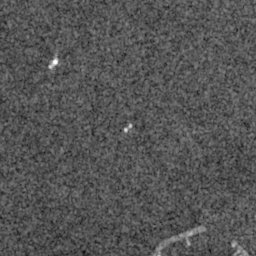
\includegraphics[width=0.38\textwidth]{detection_kish} &
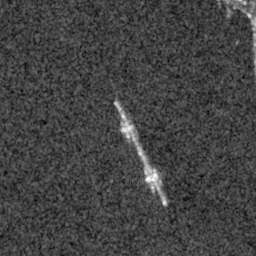
\includegraphics[width=0.38\textwidth]{persistent_kharg_jetty} \\
\small (الف) آشکارسازی مدل نزدیک کیش & \small (ب) اسکله نفتی خارک \\[4pt]
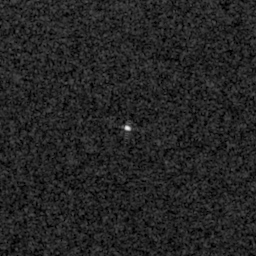
\includegraphics[width=0.38\textwidth]{persistent_assaluyeh} &
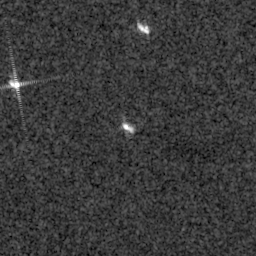
\includegraphics[width=0.38\textwidth]{persistent_bushehr} \\
\small (ج) پژواک نقطه‌ای پایدار نزدیک عسلویه & \small (د) پژواک‌های پایدار نزدیک بوشهر \\
\end{tabular}
\caption[برش‌های راداری آشکارسازی‌ها]{برش‌های راداری آشکارسازی‌ها در کنسول (قطبش \lr{VV}، شمال بالا، پهنای
\LRE{2٫56} کیلومتر، آشکارسازی در مرکز). (ب) تا (د) نقطه‌هایی‌اند که مدل در گذرهای بسیار در
آن‌ها چیزی می‌یابد؛ \lr{GFW} آن‌ها را سازه می‌شمارد و گزارش نمی‌کند.}
\label{fig:chips}
\end{figure}

قاعده نقطه پایدار (بخش~\ref{sec:persistence}) روی ۲۲۵ گذر-محدوده بایگانی \LRE{44} نقطه یافت.
نقاب کردن این نقطه‌ها روی گذرهای سپتامبر ۲۰۲۶ دقت مدل دور از ساحل ایران را از
\persistPrecisionBefore{} به \persistPrecisionAfter{} رساند، بی‌آنکه بازیابی کم شود
(جدول~\ref{tab:persistence}). اثر کوچک است: تنها حدود \LRE{6}٪ هشدارهای نادرست حذف شد، چون
بیشتر نقطه‌های تکرارشونده ۲۰۲۶ در بایگانی ۲۰۲۴ و ۲۰۲۵ نبودند. نقطه پایدار از گذرهای اخیر
باید ساخته شود؛ کنسول این آشکارسازی‌ها را علامت می‌زند و پنهان نمی‌کند.

\begin{table}[htbp]
\centering
\small
\begin{adjustbox}{max width=\textwidth}
\begin{tabular}{lcccc}
\toprule
مجموعه & امتیازدهی & دقت & بازیابی & \lr{F1} \\
\midrule
امارات، سپتامبر ۲۰۲۶ & استاندارد & \LRE{0٫591} ← \LRE{0٫594} & \LRE{0٫924} ← \LRE{0٫923} & \LRE{0٫721} ← \LRE{0٫723} \\
 & دور از ساحل & \LRE{0٫591} ← \LRE{0٫595} & \LRE{0٫924} ← \LRE{0٫924} & \LRE{0٫721} ← \LRE{0٫724} \\
ایران، سپتامبر ۲۰۲۶ & استاندارد & \LRE{0٫499} ← \LRE{0٫516} & \LRE{0٫905} ← \LRE{0٫905} & \LRE{0٫644} ← \LRE{0٫657} \\
 & دور از ساحل & \LRE{0٫509} ← \LRE{0٫523} & \LRE{0٫909} ← \LRE{0٫909} & \LRE{0٫652} ← \LRE{0٫664} \\
\bottomrule
\end{tabular}
\end{adjustbox}
\caption[اثر نقاب نقطه‌های پایدار]{اثر نقاب «نقطه‌های پایدار» (ساخته‌شده از گذرهای \lr{S1A} پیش از تیر ۱۴۰۵) روی گذرهای سپتامبر ۲۰۲۶، جداشده در زمان: پیش ← پس از حذف آشکارسازی‌های نزدیک نقطه‌ها؛ مرجع \lr{GFW} دست‌نخورده می‌ماند. «دور از ساحل»: خانه‌های بیش از ۱ کیلومتر از خشکی.}
\label{tab:persistence}
\end{table}


\section{نامزدهای شناور تاریک}
تلفیق خانه-ساعت (بخش~\ref{sec:fusion}) روی همه گذرهای سنجیده اجرا شد
(جدول~\ref{tab:dark}). روی گذرهای آزمون \darkUaeTest{} آشکارسازی‌های نگه‌داشته تاریک بودند، با
بیشترین نرخ در ناحیه هرمز. تلفیق ما با تطبیق خود \lr{GFW} سازگار است: از آشکارسازی‌هایی که
\lr{GFW} نیز بی‌\lr{AIS} می‌داند \LRE{36}٪ (\LRE{70} از \LRE{196}) تاریک شدند، و از آشکارسازی‌هایی
که \lr{GFW} با \lr{AIS} تطبیق داده تنها \LRE{2٫1}٪ (\LRE{74} از \LRE{3٬600}). نرخ تاریک با
بزرگ‌تر کردن حاشیه دروازه به‌سرعت کم می‌شود (شکل~\ref{fig:margin})؛ نامزدهایی که با حاشیه ۲
کیلومتر هم تاریک می‌مانند، اطمینان «زیاد» می‌گیرند.

\begin{table}[htbp]
\centering
\small
\begin{adjustbox}{max width=\textwidth}
\begin{tabular}{lccccc}
\toprule
مجموعه & گذر-محدوده & آشکارسازی نگه‌داشته & نرخ تاریک & بازه ۹۵٪ & داخلی / هرمز / عمان (٪) \\
\midrule
اعتبارسنجی & \LRE{25} & \LRE{1٬288} & \LRE{4٫0}٪ & \LRE{2٫6} تا \LRE{5٫8} & \LRE{6٫5} / \LRE{9٫2} / \LRE{2٫2} \\
آزمون & \LRE{92} & \LRE{4٬747} & \LRE{4٫0}٪ & \LRE{3٫2} تا \LRE{5٫3} & \LRE{7٫0} / \LRE{16٫8} / \LRE{1٫8} \\
\lr{S1A} ۲۰۲۶ & \LRE{21} & \LRE{1٬001} & \LRE{27٫8}٪ & \LRE{4٫7} تا \LRE{61٫3} & \LRE{27٫3} / \LRE{16٫7} / \LRE{28٫5} \\
\lr{S1C/D} & \LRE{42} & \LRE{2٬483} & \LRE{7٫9}٪ & \LRE{6٫3} تا \LRE{9٫7} & \LRE{18٫4} / \LRE{90٫9} / \LRE{5٫4} \\
\bottomrule
\end{tabular}
\end{adjustbox}
\caption[نرخ نامزد شناور تاریک]{نرخ نامزد شناور تاریک (تلفیق خانه-ساعت با حضور ساعتی \lr{AIS} از \lr{GFW}، حاشیه صفر متر که روی اعتبارسنجی برگزیده شد). اعتبارسنجی و آزمون: \lr{Sentinel-1A} ۲۰۲۴–۲۰۲۵؛ \lr{S1A} ۲۰۲۶: نیمه نخست ۲۰۲۶؛ \lr{S1C/D}: \lr{Sentinel-1C/1D} سپتامبر ۲۰۲۶. ستون آخر: خلیج داخلی، تنگه هرمز و دریای عمان. بازه‌ها با بوت‌استرپ روی برداشت‌ها.}
\label{tab:dark}
\end{table}


\begin{figure}[htbp]
\centering
\begin{tikzpicture}
\begin{axis}[
  width=0.8\textwidth, height=6cm,
  xmin=0, xmax=6, ymin=0, ymax=8.5,
  xtick={0,1,2,3,4,5,6},
  xticklabels={0, 250, 500, 1000, 2000, 5000, 10000},
  xlabel={\rl{حاشیه دروازه (متر)}}, ylabel={\rl{نرخ تاریک (٪)}},
  legend pos=north east, legend cell align=right,
  grid=major, grid style={gray!25},
]
\addplot[blue!70!black, thick, mark=*] table[x expr=\coordindex, y=test] {../data/dark_margin.csv};
\addlegendentry{\rl{آزمون \lr{S1A} ۲۰۲۴–۲۰۲۵}}
\addplot[orange!80!black, thick, mark=square*] table[x expr=\coordindex, y=s1cd] {../data/dark_margin.csv};
\addlegendentry{\rl{\lr{S1C/S1D} سپتامبر ۲۰۲۶}}
\end{axis}
\end{tikzpicture}
\caption[نرخ تاریک بر حسب حاشیه دروازه]{نرخ نامزد تاریک بر حسب حاشیه دروازه. حاشیه کاری (صفر متر) روی اعتبارسنجی برگزیده
شد.}
\label{fig:margin}
\end{figure}

نرخ نیمه نخست ۲۰۲۶ (\darkUaeEarly{}، با بازه‌ای بسیار پهن) از بقیه جداست: در ژانویه و فوریه
\LRE{3٫2}٪ و از مارس تا ژوئن \LRE{49}٪ بود. شکل~\ref{fig:aistrend} دلیل را نشان می‌دهد: از مارس
۲۰۲۶ ساعت-شناورهای حضور \lr{AIS} در خلیج فارس تقریباً نصف شد و سهم آشکارسازی‌های راداری
\lr{GFW} که با \lr{AIS} تطبیق می‌یابند هم‌زمان افتاد، در حالی که شمار آشکارسازی‌های راداری
تقریباً ثابت ماند. پس شناورها در دریا بودند ولی \lr{AIS} آن‌ها دیده نمی‌شد. نرخ تاریک در این دوره بیش
از رفتار شناورها، از دست رفتن پوشش \lr{AIS} را می‌سنجد؛ اخلال گسترده \lr{GNSS} در منطقه در
۲۰۲۵ و ۲۰۲۶ یک توضیح ممکن است که در این پژوهش آزموده نشد.

\begin{figure}[htbp]
\centering
\begin{tikzpicture}
\begin{axis}[
  width=0.95\textwidth, height=5.5cm,
  xmin=0, xmax=32, ymin=0, ymax=0.85,
  xtick={0,6,12,18,24,30},
  xticklabels={\lr{2024-01}, \lr{2024-07}, \lr{2025-01}, \lr{2025-07}, \lr{2026-01}, \lr{2026-07}},
  tick label style={font=\footnotesize},
  ylabel={\rl{سهم تطبیق‌یافته با \lr{AIS}}},
  legend pos=south west, legend cell align=right,
  grid=major, grid style={gray!25},
]
\addplot[blue!70!black, thick, mark=*, mark size=1pt] table[x=i, y=west] {../data/ais_trend.csv};
\addlegendentry{\rl{غرب ۵۶ درجه شرقی}}
\addplot[orange!80!black, thick, dashed, mark=square*, mark size=1pt] table[x=i, y=east] {../data/ais_trend.csv};
\addlegendentry{\rl{شرق ۵۶ درجه شرقی}}
\end{axis}
\end{tikzpicture}

\begin{tikzpicture}
\begin{axis}[
  width=0.95\textwidth, height=4.5cm,
  xmin=0, xmax=32, ymin=0, ymax=170,
  xtick={0,6,12,18,24,30},
  xticklabels={\lr{2024-01}, \lr{2024-07}, \lr{2025-01}, \lr{2025-07}, \lr{2026-01}, \lr{2026-07}},
  tick label style={font=\footnotesize},
  ylabel={\rl{هزار ساعت-شناور در روز}},
  grid=major, grid style={gray!25},
]
\addplot[teal, thick, mark=*, mark size=1pt] table[x=i, y=hours] {../data/ais_trend.csv};
\end{axis}
\end{tikzpicture}
\caption[روند حضور \lr{AIS} در خلیج فارس]{بالا: سهم آشکارسازی‌های راداری \lr{GFW} در خلیج فارس که با \lr{AIS} تطبیق یافته‌اند،
ماهانه. افت شرق از اکتبر ۲۰۲۵ خطای گذر \LRE{02:07} \lr{GFW} است؛ افت هر دو از مارس ۲۰۲۶ واقعی است.
پایین: حضور \lr{AIS} (ساعت-شناور در روز).}
\label{fig:aistrend}
\end{figure}

در ساحل ایران، روی تازه‌ترین گذری که حضور \lr{AIS} آن منتشر شده بود (۲۵ تا ۳۰ سپتامبر ۲۰۲۶)،
\LRE{109} آشکارسازی به دست آمد که \LRE{90} از پالایه‌ها گذشتند و \LRE{56} نامزد تاریک شدند:
بندرعباس ۳۳، بوشهر ۱۲، لارک/هرمز ۷، خارک ۲، کیش ۱، عسلویه ۱ و جاسک صفر (اطمینان زیاد ۱۶،
متوسط ۲۸، کم ۱۲). \lr{GFW} در خانه \LRE{32} نامزد آشکارسازی بدون \lr{AIS} دارد، در \LRE{19} خانه
چیزی ندارد و \LRE{5} نامزد را با \lr{AIS} تطبیق داده است. \LRE{24} نامزد در نقطه‌هایی‌اند که
در دست‌کم سه گذر دیگر نیز آشکارسازی داشته‌اند و ممکن است سازه یا شناور لنگرانداخته باشند.
در شش محدوده از هفت، شمار شناورهای تطبیق‌یافته \lr{GFW} برای داوری درباره کامل بودن حضور
\lr{AIS} کافی نبود؛ پس این شمارش‌ها نامزدند، نه یافته.

\section{کارایی}
روی پردازنده رایانه همراه این پژوهش (\lr{Ryzen 7 3700U}، بدون \lr{GPU})، اجرای مدل روی پنجره
\benchWindow{}$\times$\benchWindow{} پیکسلی یک محدوده ۲۰ کیلومتری به‌طور میانه \benchSeconds{} ثانیه
طول کشید، با بیشینه حافظه \benchMemory{} مگابایت. میانگین زمان مدل روی گذرهای واقعی آزمون
\testModelSeconds{} ثانیه بود (آبراه هرمز ۴۰ کیلومتری حدود چهار برابر یک محدوده ۲۰ کیلومتری
است). در اجرای ساحل ایران، هر محدوده از جست‌وجو تا ذخیره حدود ۳۰ تا ۴۰ ثانیه طول کشید و
هر درخواست حضور \lr{AIS} از \lr{GFW} حدود ۲۰ ثانیه؛ پس مدل تنگنای سامانه نیست.

\chapter{بحث و نتیجه‌گیری}
\label{ch:conclusion}

\section{جمع‌بندی یافته‌ها}
\begin{enumerate}
\item یک آشکارساز نقطه‌ای یادگیری عمیق را می‌توان بدون حتی یک برچسب دستی، با برچسب‌هایی که
از کنار هم گذاشتن \lr{CFAR} و آشکارسازی‌های منتشرشده \lr{GFW} ساخته می‌شود، برای یافتن
شناور در تصاویر \lr{Sentinel-1} آموزش داد و روی پردازنده یک رایانه همراه اجرا کرد (حدود
\benchSeconds{} ثانیه برای یک محدوده ۲۰ کیلومتری).
\item برچسب‌های خودکار سوگیری دارند. مدلی که تنها از شناورهای دارای \lr{AIS} آموخت، نیمی از
شناورهای بدون \lr{AIS} را از دست داد (\darkRecallRunOne{} در برابر \darkRecallCfar{} برای
\lr{CFAR})؛ برای سامانه‌ای که هدفش یافتن شناور تاریک است، این بدترین خطای ممکن است. افزودن
آشکارسازی‌های بدون \lr{AIS} به مثبت‌ها آن را برطرف کرد (\darkRecallModel).
\item روی ۹۲ گذر آزمون نگه‌داشته، مدل نهایی اندکی بهتر از \lr{CFAR} بود (\lr{F1}
\testFOneModel{} در برابر \testFOneCfar{}، تفاضل \testDiffCi). برتری کوچک ولی معنادار است.
\item مدل بدون بازتنظیم به ماهواره‌های تازه \lr{Sentinel-1C/1D} و به ساحل ایران تعمیم یافت.
برتری بزرگ ظاهری آن نزدیک ساحل از نوار یک‌کیلومتری‌ای می‌آید که مرجع در آن گزارشی ندارد؛
دور از ساحل برتری کوچک اما معنادار می‌ماند.
\item بخش بزرگی از «هشدارهای نادرست» در ساحل ایران سازه‌های واقعی‌اند که مرجع آن‌ها را حذف
کرده است؛ دقت گزارش‌شده آنجا کرانی پایین است.
\item تلفیق خانه-ساعت با حضور ساعتی \lr{AIS} نرخ نامزد تاریک را با روشی یکسان در دوره‌ها و
منطقه‌ها می‌سنجد و با تطبیق خود \lr{GFW} سازگار است. اما نرخ تاریک هم رفتار شناورها را
می‌سنجد و هم کامل بودن پوشش \lr{AIS} را: جهش آن در بهار ۲۰۲۶ با نصف شدن حضور \lr{AIS}
هم‌زمان است.
\end{enumerate}

\section{محدودیت‌ها}
\begin{itemize}
\item \textbf{مرجع، حقیقت زمینی نیست.} همه سنجش‌ها در برابر \lr{GFW} است که آشکارساز و خطاهای
خودش را دارد، روی \lr{Sentinel-1C/1D} کم‌پشت‌تر است، در نوار ساحلی چیزی گزارش نمی‌کند و یک
گذر را به‌اشتباه بی‌\lr{AIS} می‌شمارد. هیچ برچسب دستی‌ای در این پژوهش نیست.
\item \textbf{تفکیک مرجع حدود ۱ کیلومتر است.} تطبیق در سطح خانه \LRE{0٫01} درجه‌ای انجام
می‌شود؛ خطای موقعیت کمتر از یک خانه سنجیده نمی‌شود و دو شناور نزدیک در یک خانه از هم جدا
نمی‌شوند.
\item \textbf{برچسب‌ها از \lr{CFAR} آمده‌اند.} مدل ممکن است چیزهایی را که \lr{CFAR} نمی‌بیند (شناور
کوچک چوبی، شناور در دریای ناآرام) نیاموخته باشد. نزدیک نیمی از مثبت‌های بدون \lr{AIS}
(\LRE{727} از \dataTrainDark) از گذرِ دچار خطای \lr{GFW} آمده‌اند و به احتمال زیاد \lr{AIS}
داشته‌اند؛ برای آموزش مشکلی نیست، چون همچنان شناورند.
\item \textbf{مدل تنها مکان را می‌دهد.} طول، جهت و نوع شناور برآورد نمی‌شود، چون برچسب
قابل‌اعتمادی برایشان نبود.
\item \textbf{تلفیق تنها حضور ساعتی دارد.} مسیر نقطه‌به‌نقطه \lr{AIS} رایگان در دسترس نبود؛ کران
\lr{R/V} ثابت گرفته شد و پالایه‌های پژواک‌های کاذب در امتداد سمت و لبه تصویر ساخته نشد.
\item \textbf{نمونه نامزدهای ایران کوچک است} و در شش محدوده از هفت، کامل بودن حضور \lr{AIS}
قابل‌داوری نبود. اخلال \lr{GNSS} در منطقه هر تلفیق با \lr{AIS} را سوگیر می‌کند.
\item \textbf{هر پیکربندی یک بار آموزش دید}؛ پراکندگی نتایج میان آموزش‌های تکراری سنجیده نشد.
\end{itemize}

\section{کارهای آینده}
\begin{itemize}
\item \textbf{برچسب دستی نزدیک ساحل:} نوار یک‌کیلومتری ساحل، که مرجع در آن خاموش است، تنها با
برچسب‌گذاری دستی یا داده‌ای دیگر سنجیدنی است.
\item \textbf{\lr{AIS} نقطه‌به‌نقطه:} داده تجاری مسیر شناورها دروازه‌ها را تنگ‌تر و نامزدها را
مطمئن‌تر می‌کند.
\item \textbf{بایگانی پایدار غلتان:} ساختن نقطه‌های پایدار از گذرهای اخیر به‌جای بایگانی ثابت.
\item \textbf{برآورد طول و نوع شناور} با برچسب‌هایی از ثبت‌های \lr{AIS}، و پالایه پژواک‌های کاذب
با هندسه هر تصویر.
\item \textbf{سنجش کاربردپذیری کنسول:} آزمودن اینکه کاربری غیرمتخصص بتواند بی‌کمک یک نامزد
شناور تاریک را بیابد و شواهدش را بخواند.
\end{itemize}

\section{سخن پایانی}
این پژوهش نشان داد که با داده‌های رایگان و یک رایانه همراه می‌توان شناورهای خلیج فارس را در
تصاویر راداری یافت و آن‌ها را با \lr{AIS} مقایسه کرد. درس اصلی آن بیش از معماری مدل، درباره
داده است: برچسبی که از \lr{AIS} بیاید، مدل را به سوی شناورهای دارای \lr{AIS} می‌کشد، و مرجعی
که سازه‌ها و ساحل را کنار می‌گذارد، عدد دقت را جابه‌جا می‌کند. سامانه‌ای که هر آشکارسازی را
با تصویر راداری‌اش و با بیان صادقانه سن داده و دقت سنجیده‌شده نشان دهد، به تحلیلگر اجازه
می‌دهد خودش داوری کند.


\renewcommand{\bibname}{مراجع}
\begin{thebibliography}{99}
\begin{latin}

\bibitem{torres2012} R.~Torres et al., ``GMES Sentinel-1 mission,''
\emph{Remote Sensing of Environment}, vol.~120, pp.~9--24, 2012.

\bibitem{cdse} European Space Agency, ``Copernicus Data Space Ecosystem.''
\url{https://dataspace.copernicus.eu}. Contains modified Copernicus Sentinel data.

\bibitem{kroodsma2018} D.~A. Kroodsma et al., ``Tracking the global footprint of
fisheries,'' \emph{Science}, vol.~359, no.~6378, pp.~904--908, 2018.

\bibitem{paolo2024} F.~S. Paolo et al., ``Satellite mapping reveals extensive
industrial activity at sea,'' \emph{Nature}, vol.~625, pp.~85--91, 2024.

\bibitem{gfwapi} Global Fishing Watch, ``APIs: 4Wings SAR vessel detections and
AIS vessel presence.'' \url{https://globalfishingwatch.org/our-apis/}.
Powered by Global Fishing Watch.

\bibitem{crisp2004} D.~J. Crisp, ``The state-of-the-art in ship detection in
synthetic aperture radar imagery,'' DSTO, Tech. Rep. DSTO-RR-0272, 2004.

\bibitem{paolo2022} F.~Paolo et al., ``xView3-SAR: Detecting dark fishing
activity using synthetic aperture radar imagery,'' in \emph{Advances in Neural
Information Processing Systems (Datasets and Benchmarks Track)}, 2022.

\bibitem{xview3first} E.~Khvedchenya, ``xView3 challenge: first place solution.''
\url{https://github.com/BloodAxe/xView3-The-First-Place-Solution} (MIT licence).

\bibitem{ronneberger2015} O.~Ronneberger, P.~Fischer, and T.~Brox, ``U-Net:
Convolutional networks for biomedical image segmentation,'' in \emph{MICCAI},
LNCS vol.~9351, pp.~234--241, 2015.

\bibitem{zhou2019} X.~Zhou, D.~Wang, and P.~Kr\"ahenb\"uhl, ``Objects as
points,'' arXiv:1904.07850, 2019.

\bibitem{tan2019} M.~Tan and Q.~V. Le, ``EfficientNet: Rethinking model scaling
for convolutional neural networks,'' in \emph{ICML}, PMLR vol.~97,
pp.~6105--6114, 2019.

\bibitem{lin2017} T.-Y. Lin, P.~Goyal, R.~Girshick, K.~He, and P.~Doll\'ar,
``Focal loss for dense object detection,'' in \emph{ICCV}, pp.~2980--2988, 2017.

\bibitem{kuhn1955} H.~W. Kuhn, ``The Hungarian method for the assignment
problem,'' \emph{Naval Research Logistics Quarterly}, vol.~2, no.~1--2,
pp.~83--97, 1955.

\bibitem{efron1993} B.~Efron and R.~J. Tibshirani, \emph{An Introduction to the
Bootstrap}. Chapman \& Hall, 1993.

\bibitem{spanier2026} Spanier, Hoeser, Truckenbrodt, Bachofer, and Kuenzer,
``Offshore Platform Dataset (OPD) v1.0.0,'' Zenodo, 2026,
doi:10.5281/zenodo.19046824 (CC BY 4.0); described in \emph{Big Earth Data}.

\bibitem{osm} OpenStreetMap contributors, ``Land polygons.''
\url{https://osmdata.openstreetmap.de/data/land-polygons.html} (ODbL).

\end{latin}
\end{thebibliography}


\begin{latin}
\chapter*{Abstract}
The Persian Gulf and the Strait of Hormuz carry some of the world's densest
shipping, yet the Automatic Identification System (AIS) by which ships report
their position is self-reported and can be switched off or spoofed. Sentinel-1
synthetic aperture radar (SAR) sees vessels whatever their AIS, cloud or
daylight. This thesis trains a deep-learning point detector (EfficientNet-B0
encoder, U-Net decoder) on Sentinel-1 images without manual labels, using
Global Fishing Watch (GFW) radar detections as the source of labels, and runs
it on a laptop CPU. A first model found vessels without AIS less often than a
classical CFAR detector, because its labels came only from AIS-broadcasting
ships; adding GFW detections without AIS as positives removed this bias. On
92 held-out test passes the final model reaches an F1 against GFW slightly
above CFAR's, transfers without recalibration to the new Sentinel-1C/1D
satellites and to the Iranian coast, and, fused with hourly AIS presence,
flags dark-vessel candidates with their evidence. A Persian web console shows
every detection with its radar image.

\noindent\textbf{Keywords:} synthetic aperture radar, Sentinel-1, deep learning,
ship detection, dark vessels, AIS, Persian Gulf.
\end{latin}

\end{document}
